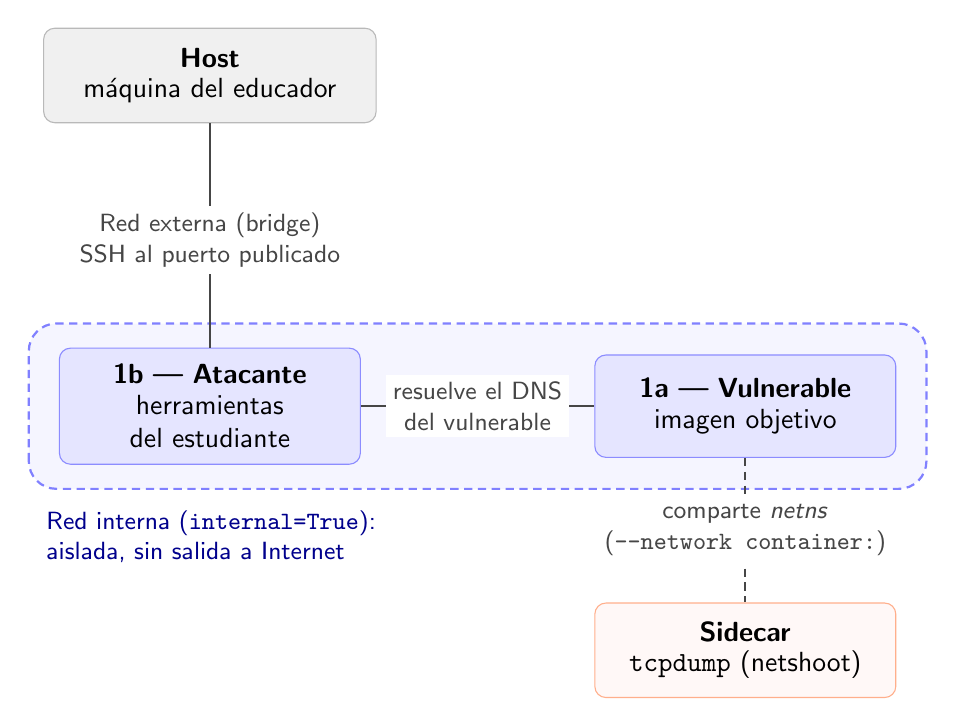
\begin{tikzpicture}[
    every node/.style={font=\sffamily},
    cont/.style={rounded corners=4pt, draw=blue!45, fill=blue!10,
                 minimum height=1.3cm, text width=3.4cm, text centered,
                 inner sep=6pt},
    host/.style={rounded corners=4pt, draw=gray!55, fill=gray!12,
                 minimum height=1.2cm, text width=3.8cm, text centered,
                 inner sep=6pt},
    side/.style={rounded corners=4pt, draw=orange!60!red!45, fill=orange!7!red!3,
                 minimum height=1.2cm, text width=3.4cm, text centered,
                 inner sep=6pt},
    link/.style={thick, gray!55!black},
    llbl/.style={font=\sffamily\small, fill=white, inner sep=2.5pt, align=center},
]
% ── Zona: red interna (dibujada primero, queda detrás) ──
\draw[draw=blue!50, densely dashed, thick, rounded corners=10pt, fill=blue!4]
    (-5.7,-1.05) rectangle (5.7,1.05);
\node[font=\sffamily\small, text=blue!55!black, anchor=north west, align=left]
    at (-5.6,-1.2)
    {Red interna (\texttt{internal=True}):\\aislada, sin salida a Internet};

% ── Host (fuera de las redes Docker) ──
\node[host] (host) at (-3.4, 4.2)
    {\textbf{Host}\\[-1pt]{\normalsize máquina del educador}};

% ── Contenedores (encima de la zona) ──
\node[cont] (atk) at (-3.4, 0)
    {\textbf{1b — Atacante}\\[-1pt]{\normalsize herramientas del estudiante}};
\node[cont] (vuln) at (3.4, 0)
    {\textbf{1a — Vulnerable}\\[-1pt]{\normalsize imagen objetivo}};
\node[side] (side) at (3.4, -3.1)
    {\textbf{\textit{Sidecar}}\\[-1pt]{\normalsize \texttt{tcpdump} (netshoot)}};

% ── Enlaces ──
% Host ↔ Atacante (red externa, bridge)
\draw[link] (host.south) -- (atk.north)
    node[llbl, pos=0.52] {Red externa (bridge)\\SSH al puerto publicado};
% Atacante ↔ Vulnerable (dentro de la red interna)
\draw[link] (atk.east) -- (vuln.west)
    node[llbl, pos=0.5] {resuelve el DNS\\del vulnerable};
% Sidecar comparte el netns del vulnerable
\draw[link, densely dashed] (vuln.south) -- (side.north)
    node[llbl, pos=0.5] {comparte \textit{netns}\\(\texttt{-{}-network container:})};
\end{tikzpicture}
